\documentclass[11pt]{article}
\usepackage{enumerate}
\usepackage{fullpage}
\usepackage{fancyhdr}
\usepackage{amsmath, amsfonts, amsthm, amssymb}
\usepackage{color}
\setlength{\parindent}{0pt}
\setlength{\parskip}{5pt plus 1pt}
\usepackage[]{graphicx}
\usepackage{subcaption}

\usepackage {tikz}
\usetikzlibrary{positioning}
\definecolor{processblue}{cmyk}{0.96,0,0,0}


%%%%%%%%%%%%%%%%%%%%%%%HEADER%%%%%%%%%%%%%%%%%%%%%%%%%%%%%%
\newcommand{\myname}{Shashank Singh\footnote{sss1@andrew.cmu.edu}}
\newcommand{\myclass}{36-757 Advanced Data Analysis I}
\newcommand{\myhwname}{ADA Project}
\newcommand{\duedate}{Wednesday, \today}
%%%%%%%%%%%%%%%%%%%%%%%%%%%%%%%%%%%%%%%%%%%%%%%%%%%%%%%%%%%

%%%%%%%%%%%%%%%%%%%%CONTENT MACROS%%%%%%%%%%%%%%%%%%%%%%%%%
\renewcommand{\qed}{\quad \ensuremath{\blacksquare}}
\newcommand{\inv}{^{-1}}
\newcommand{\dist}{\operatorname{dist}}
\newcommand{\area}{\operatorname{area}}
\newcommand{\vspan}{\operatorname{span}}
\newcommand{\Gr}{\operatorname{Gr}} % graph of a function
\renewcommand{\sp}{\operatorname{span}} % span of a set
\newcommand{\sminus}{\backslash}
\newcommand{\E}{\mathbb{E}} % expected value
\newcommand{\F}{\mathcal{F}}
\newcommand{\X}{\mathcal{X}}
\newcommand{\Y}{\mathcal{Y}}
\newcommand{\Z}{\mathcal{Z}}
\newcommand{\pr}{\mathbb{P}} % probability
\newcommand{\Var}{\mathbb{V}} % variance
\newcommand{\Cov}{\operatorname{Cov}} % covariance
\newcommand{\pow}[1]{\mathcal{P}\left(#1\right)} % power set of #1
\newcommand{\e}{\varepsilon} % \varepsilon
\renewcommand{\P}{\mathbb{P}}   % probability
\newcommand{\ol}{\overline}
%%%%%%%%%%%%%%%%%%%%%%%%%%%%%%%%%%%%%%%%%%%%%%%%%%%%%%%%%%%

\begin{document}
\thispagestyle{plain}

{\Large \myhwname} \\
Name: \myname \\
\myclass \\
\duedate

\section{Project Introduction}
Internal Advisor: Barnab\'as P\'oczos, Assistant Professor, Machine Learning
Department  \\
External Advisor: Timothy Verstynen, Assistant Professor, Psychology
Department  \\
Tentative Title: Inferring Higher-Order Functional Connectivity in fMRI

{\bf fMRI and BOLD Signal:}
fMRI is a whole-brain imaging modality that measures BOLD (blood-oxygen-level
dependent) signal. BOLD signal is a measure of the oxygenated blood flow to a
region, which increases as a response to increased metabolic demand in that
region (hemodynamic response). Thus, BOLD signal is measured as a surrogate for
brain activity. fMRI measures BOLD signal within each cell (known as a
\emph{voxel}) of a fine 3-dimensional grid in which the brain rests, roughly
once per second. Thus, fMRI is used to measure activity in precise regions
throughout the brain with high spatial resolution (on the order of
millimeters), albeit with low temporal resolution relative to the dynamics of
neurons, which can signal hundreds on times per second.

A major application of fMRI is in estimating \emph{functional connectivity},
DEFINE.

The goal of this project is to evaluate methods for measuring functional
connectivity in fMRI data. In particular, we would like effective methods for
inferring higher-order connectivity; that is, we would like to distinguish pairs
of regions that are ``directly'' functionally connected from those for which
the connectivity can be explained by functional connectivity between
intermediate regions).

\begin{figure}[h]
\centering
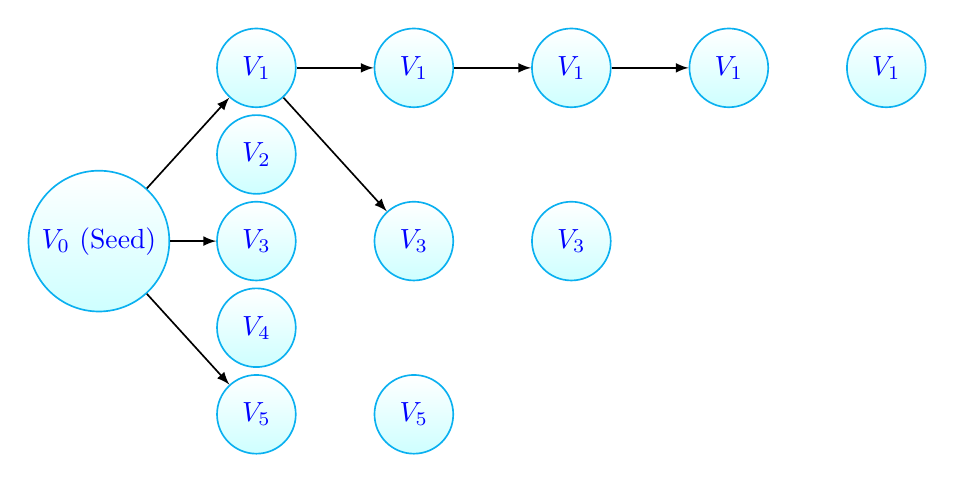
\begin{tikzpicture}[-latex, auto, node distance=4 cm and 5cm, on grid,
semithick, state/.style={circle, top color=white, bottom color=processblue!20,
draw, processblue, text=blue, minimum width=1 cm}]
  % seed
  \node[state] (n0) at (1,5) {$V_0$ (Seed)};
  % layer 1
  \node[state] (n11) at (3,2.8)  {$V_5$};
  \node[state] (n12) at (3,3.9)  {$V_4$};
  \node[state] (n13) at (3,5)    {$V_3$};
  \node[state] (n14) at (3,6.1)  {$V_2$};
  \node[state] (n15) at (3,7.2)  {$V_1$};
  % layer 2
  \node[state] (n21) at (5,2.8)  {$V_5$};
  \node[state] (n23) at (5,5)    {$V_3$};
  \node[state] (n25) at (5,7.2)  {$V_1$};
  % layer 3
  \node[state] (n33) at (7,5)    {$V_3$};
  \node[state] (n35) at (7,7.2)  {$V_1$};
  % layer 4
  \node[state] (n45) at (9,7.2)  {$V_1$};
  % layer 5
  \node[state] (n55) at (11,7.2) {$V_1$};

\foreach \from/\to in {n0/n15,n0/n13,n0/n11,n15/n25,n15/n23,n25/n35,n35/n45}
    \draw (\from) -- (\to);
\end{tikzpicture}
\caption{An example sequence of conditional dependencies amongst voxels. V2 and
V4 are independent of the seed, while V1, V3, and V5 are not. V5 is
conditionally independent of the seed given ???}
\end{figure}

\section{Description of Data and Basic EDA}
Each of 60 subjects (30 males, 30 females, ages 19-29) was scanned on a 3T
Siemens Verio at the Scientific Imaging \& Brain Research Center at CMU.
Participants remained in a resting state.

For each subject, the main object of the data is a length $T = 200$ time series
of BOLD signal in each of $V = 160,990$ voxels. Specifically, for each subject,
we have a $V \times T$ matrix.

The 160,990 voxels comprise $600$ known regions of interest (ROIs), and one way
to reduce the data's dimensionality may be to aggregate data within these ROIs
to produce a $600$ dimensional time series. For each voxel, spatial ($xyz$)
coordinates are also known.

We first perform some basic denoising and normalization on the raw data.
Denoising consists of removing large slow-wave oscillations via PCA by
computing the first $3$ eigenvectors of the signal, reconstructing the signal
from those three eigenvectors, and then subtracting the result from the
original signal. We then normalize the data by $Z$-scoring, so that each voxel
has mean $0$ and standard deviation $1$ over time. An example of the resulting
data is given in Figure \ref{fig:eda}.

%%%BEGIN FIGURE%%%
\begin{figure}[h!]
\begin{subfigure}{.5\textwidth}
  \centering
  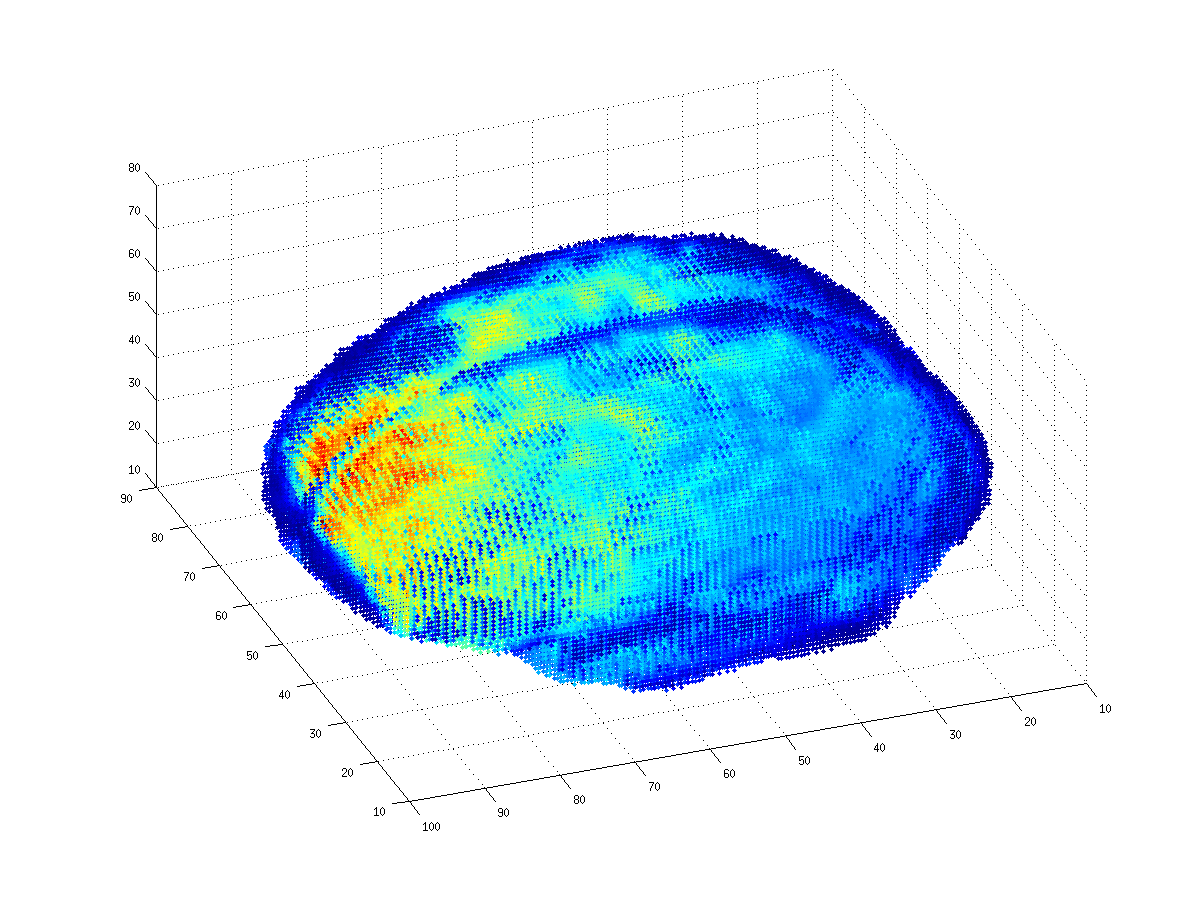
\includegraphics[width=\linewidth]{eda1}
  \caption{1a}
  \label{fig:eda_all}
\end{subfigure}%
\begin{subfigure}{.5\textwidth}
  \centering
  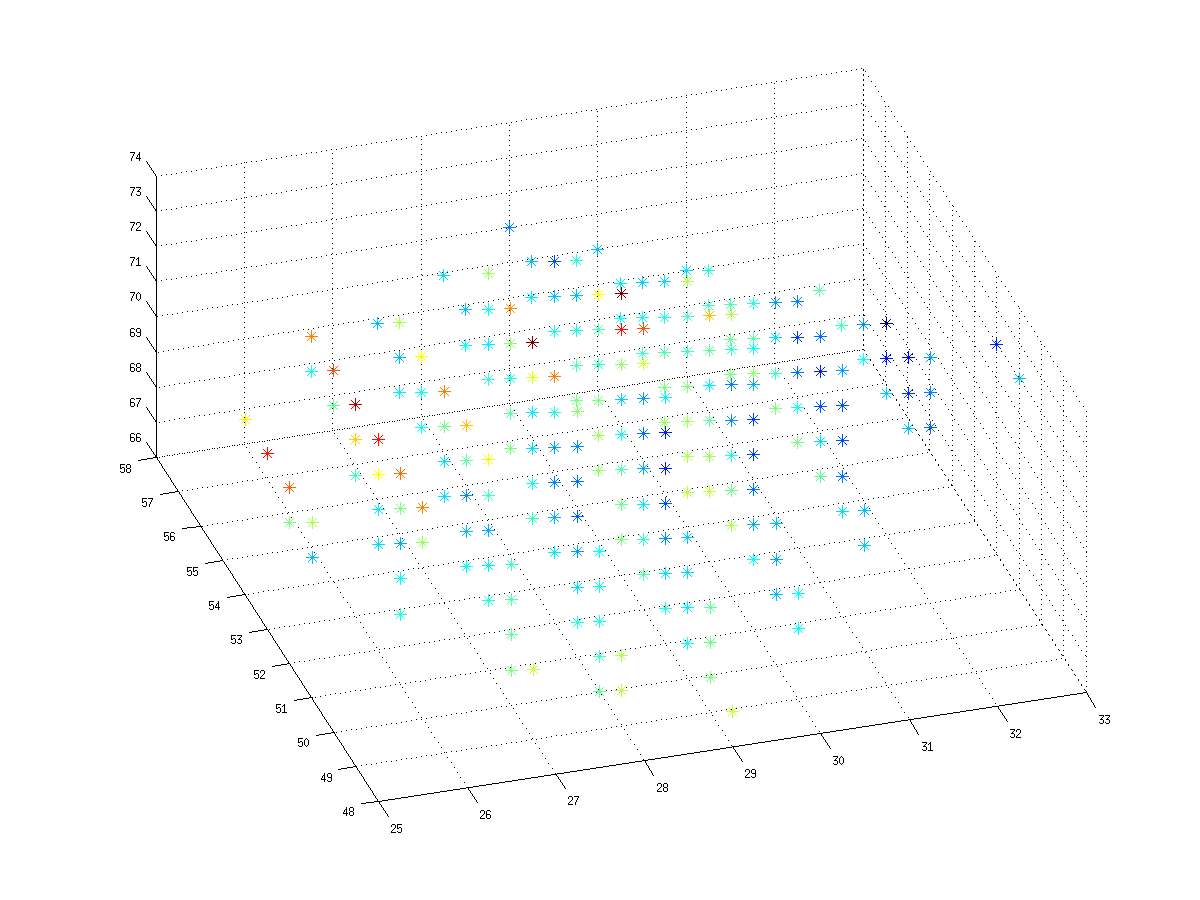
\includegraphics[width=\linewidth]{eda2}
  \caption{1b}
  \label{fig:eda_ROIs}
\end{subfigure}
\caption{BOLD signals for a single time frame from a single subject for all
voxels (\ref{fig:eda_all}) and for all ROIs, averaged over voxels in each ROI
(\ref{fig:eda_ROIs}).}
\label{fig:eda}
\end{figure}
%%%%%END FIGURE%%%

\section{Statistical Formulation}
One statistical framework that approximates our problem is learning a graphical
model over the voxels.

This can be thought of as learning a minimal
\footnote{In the sense of having no unnecessary edges.}
graphical model whose variables are activity levels of brain regions.

In addition to utilizing established methods such as variants of regularized
linear regression and correlation, we would like to we would like to explore
some more recently proposed methods, such a information-theoretic approaches, to
see whether they can better measure functional connectivity (for example, by
capturing nonlinear dependence or conditioning).

\section{Related Work}
\cite{Grosenick13GraphNet}, \cite{Li09FDRinPCAlgo}, \cite{Garg11FARM},

However, that the limitations of fMRI, and in particular of the BOLD signal,
must be considered when measuring functional connectivity. For example, a
recent meta-analysis of various fMRI studies, \cite{webb13grangerVascular},
studied the use of Granger causality to measure functional connectivity, and
found that Granger Causality was strongly predicted by brain vasculature. This
suggests that, rather than

One response has been that researches should not consider measuring functional
connectivity for its own sake, and that functional connectivity should only be
analyzed differentially; that is, functional connectivity should only be
studied in terms of how it differs

Over a large collection of data sets, they showed that whether a voxel $A$
Granger causes another voxel $B$ is strongly influenced by ambient vascular
anatomy. In particular, $A$ is systematically more likely than otherwise to
Granger cause $B$ if $A$ is a vascular source, $B$ was a vascular sink, or
both. More generally, this suggests that, default-state blood flow may
sometimes have a stronger effect on Granger causality \footnote{or any other
method) which measures directed functional connectivity by measuring the
predictive power of a voxel on another voxel later in time.} of BOLD signals
than actual neural activity.

\cite{Craddock13predictingBrain},
\cite{Carroll09predictBrainDistributedSparse},
\cite{Ryali12stabilityElasticNet}
\section{Proposed Methodologies}

\begin{table}
\centering
\begin{tabular}{|r|c|c|c|c|}
\hline
            & \multicolumn{2}{|c|}{Parametric (Linear)} & \multicolumn{2}{|c|}{Semi/Nonparametric} \\ % <---- inserted &
\hline
            & Prediction-Based                          & Similarity-Based  & Prediction-Based  & Similarity-Based      \\
\hline                                                                                                                  
Time Series & Granger Causality                         & Cross-Correlation & Transfer Entropy  & Cross-Information     \\
\hline                                                                                                                    
IID         & Elastic Net                               & Correlation       & Nonpar Regression & Mutual Information    \\
            & LASSO                                     &                   & FuSSO             &                       \\
\hline
\end{tabular}
\caption{Conceptual breakdown of several of the dependence measures we
consider.}
\label{tab:methods}
\end{table}

\subsection{Regression Based Methods}
\subsubsection{LASSO, Ridge, and Elastic Net}
One way of measuring the relative dependence of a variable $Y$ on other
variables $X$ is to regress $Y$ over $X$. When using all $160,990$ voxels,
ordinary least squares (OLS) is out of the question ($p \gg n$). The automatic
variable selection performed by $L_1$ regularization (LASSO) is desirable and
easily interpretable in our context; voxels selected are considered to be
functionally connected to the seed voxel. However, because we would like to be
able to select more than $n$ voxels, and also because we also expect
multicollinearity amongst nearby voxels, $L_2$ regularization (ridge) is also
desirable. Hence, we propose to use elastic net regularization, a weighted
combination of $L_1$ and $L_2$ regularization. Specifically, we will use the
elastic net regression implementation in the MATLAB package \texttt{glmnet}.

\subsubsection{Group LASSO}

\subsection{Dependence Measure Based Methods}
\subsubsection{Linear Methods}
{\bf Correlation:} Perhaps the simplest way of measuring dependence is
estimating the correlation
$\rho(V_i,V_j) = \frac{\operatorname{Cov}[V_i,V_j]}{\Var[V_i]\Var[V_j]}$.

{\bf Cross-Correlation:} Correlation fails to take into account the time series
nature of fMRI data.

{\bf Granger Causality:}

Previous work [CITATION NEEDED] has noted that Granger Causality is affected by
the vascular structure of the brain, which is independent of the functional
activity we are trying to measure. For example, certain brain regions which
serve as oxygenated blood sources tend to appear as Granger causal, while
regions which serve as blood sinks tend to appear as Granger consequentail.

\subsubsection{Mutual Information and Conditional Mutual Information}
For two random variables $X$ and $Y$ taking values in $\X$ and $\Y$,
respectively, the \emph{Shannon mutual information} $I(X;Y)$ between $X$ and
$Y$ is defined as
\[I(X;Y)
    := \int_{\X \times \Y} p(x,y) \log \frac{p(x,y)}{p(x)p(y)}
    = \E_{X,Y} \left[ \log \frac{p(X,Y)}{p(X)p(Y)} \right],
\]
where $p$ denotes the appropriate (marginal or joint) density function in each
instance. For a third random variable $Z$ taking values in $\Z$, the
\emph{conditional Shannon mutual information} $I(X;Y|Z)$ between $X$ and $Y$
given $Z$ is defined as
\begin{align*}
I(X;Y|Z)
 &  := \int_\Z p(z) \int_{\X \times \Y}
                p(x,y|z) \log \frac{p(x,y|z)}{p(x|z)p(y|z)} \, d(x,y) \, dz \\
 &  = \int_{\X \times \Y \times \Z}
                    p(x,y,z) \log \frac{p(x,y,z)p(z)}{p(x,z)p(y,z)} \, d(x,y,z)
    = \E_{X,Y,Z} \left[ \log \frac{p(X,Y)}{p(X)p(Y)} \right],
\end{align*}
Intuitively, $I(X;Y)$ is a measure of dependence between $X$ and $Y$ (for
example, if $X$ and $Y$ are Gaussian, then is a (strictly) increasing function
of the absolute value of the correlation $|\rho(X,Y)|$), and hence $I(X;Y|Z)$
is a measure of dependence between $X$ and $Y$ conditioned on $Z$. Furthermore,
two classic results in information theory are that $I(X;Y) = 0$ if and only if
$X \perp Y$ and that $I(X;Y|Z) = 0$ if and only if $X \perp Y | Z$.

In fact, if we can estimate $I(X;Y)$ with $(1 - \alpha)$ confidence intervals,
we can formally test the null hypothesis $X \perp Y$ with Type I error
probability $\alpha$, and, similarly, estimating $I(X;Y|Z)$ with confidence
leads to a test of the null $X \perp Y | Z$. In our case, such a test can be
used as a component of a procedure such as the PC algorithm
\cite{spirtes2000causation} for learning graphical models.

\subsection{Parameter Selection}
Each of the methods discussed above has some real-valued parameter that trades
off our false-positive and false negative rates. For methods with formal tests,
such as Granger causality and the PC algorithm, this is simply the Type I error
probability, although, due to multiple testing, it may be preferable to use the
false discovery rate (FDR) (see, e.g., \cite{Li08connectivityFDRcontrolledPC}
for a method of controlling FDR in the PC algorithm).

For similarity measures (, this is a threshold, above which


this is simply the false positive rate $\alpha$ 

For similarity based methods, such as (cross-)correlation 
Granger Causality


\section{Visualization}
The high dimensional nature of fMRI data makes visualizing results quite
difficult. This even worse when we are studying connectivity, because there are
$\frac{n(n - 1)}{2}$ possible pairwise connections over $n$ voxels. Here, we
discuss some basic approaches to visualizing fMRI data.

\subsection{Brain-Like Visualizations}
For biological interpretation, it would be desirable to preserve the relative
positions of voxels or ROIs within the brain. When plotting all voxels, one
brain-like

\section{Graphical Model Approaches}
\subsection{Chow-Liu Approximation}

\subsection{PC Algorithm}

\section{Observations, Ideas, Attempts, and Other Notes}
From the full dataset, \texttt{0006\_AAL3.mat}, I first extracted the relevant
components of the data from the raw fMRI \texttt{.mat} files into my own
reduced format as follows:
\begin{verbatim}
load 0006_AAL3;
n = length(dat_obj.vox_info);
data = double(dat_obj.data');
for i = 1:n,
  rois(i) = dat_obj.vox_info(i).val;
  XYZ(:, i) = dat_obj.vox_info(i).XYZ;
end
save('my_AAL3.mat', 'data', 'n', 'rois', 'XYZ');
\end{verbatim}
Computing the covariance BLAHBLAHBLAH

\section{Stepwise Approaches}
Suppose we want to distinguish different orders of connectivity; that is, if
a voxel $C$ is connected to a voxel $A$ through another voxel $B$, but $C$ is
not connected directly to $A$, we would like distinguish this from the case
that $C$ is connected directly to $A$.

Given a seed voxel $s$, one approach to determining the order of connectivity
might be the following:
\begin{enumerate}
\item Initialize a collection $C$ with all voxels.
\item Remove from $C$ any voxel which is (unconditionally) independent of $s$.
\item For each voxel, remove any voxels 
\end{enumerate}

\subsection{Future Work}
\begin{enumerate}
\item Run the PC algorithm on the (likely reduced) data, using my CMI estimator
\item Talk to Barnabas and Tim about how exactly to condition edges in one
layer on edges in previous layers
\item Try decorrelating some (synthetic and fMRI) time series, and running a
(conditional) mutual information estimator on them
\item Try running a transfer entropy estimator (under a Markov assumption) on
some (synthetic and fMRI) time series
\item Try estimating the limit of a sequence of biased estimates with
increasing sample sizes to reduce the bias of the estimator
\item Also try undersmoothing or using the von Mises correction to reduce the
bias of the estimator
\item Ask Tim whether it could be realistic to bound the degree of each voxel;
if so, perhaps we can apply the algorithm Samy, Akshay, and Larry are working
on?
\item Consider within-ROI and without-ROI edges separately?
\end{enumerate}

{\small
\bibliographystyle{plain}
\bibliography{biblio}
}

\end{document}
